\chapter{Global image features}
The task in this tutorial is to understand how we can extract numerical representations from images 
and how these numerical representations can be used to provide similarity measures between images, 
so that we can, for example, find the most similar images from a set.

As you know, images are made up of pixels which are basically numbers that represent a colour. 
This is the most basic form of numerical representation of an image. However, we can do calculations 
on the pixel values to get other numerical representations that mean different things. In general, 
these numerical representations are known as \textbf{feature vectors} and they represent particular 
\textbf{features}.

Let's take a very common and easily understood type of feature. It's called a colour histogram and 
it basically tells you the proportion of different colours within an image (e.g. 90\% red, 5\% green, 
3\% orange, and 2\% blue). As pixels are represented by different amounts of red, green and blue we 
can take these values and accumulate them in our histogram (e.g. when we see a red pixel we add 1 
to our `red pixel count' in the histogram). 

A histogram can accrue counts for any number of colours in any number of dimensions but the usual 
is to split the red, green and blue values of a pixel into a smallish number of `bins' into which the 
colours are thrown.  This gives us a three-dimensional cube, where each small cubic bin is accruing 
counts for that colour.

OpenIMAJ contains a multidimensional \verb+Histogram+ implementation that is constructed using the number 
of bins required in each dimension. For example:
\begin{lstlisting}[language=java]
Histogram histogram = new Histogram( 4, 4, 4 );
\end{lstlisting}
This code creates a histogram that has 64 ($4\times4\times4$) bins. However, this data structure does not do 
anything on its own. The \verb+HistogramModel+ class provides a means for creating a \verb+Histogram+ 
from an image.  The \verb+HistogramModel+ class assumes the image has been normalised and returns a normalised histogram:
\begin{lstlisting}[language=java]
HistogramModel model = new HistogramModel( 4, 4, 4 );
model.estimateModel( image );
Histogram histogram = model.histogram;
\end{lstlisting}

You can print out the histogram to see what sort of numbers you get for different images. 
Let's load in 3 images then generate and store the histograms for them:
\marginpar{
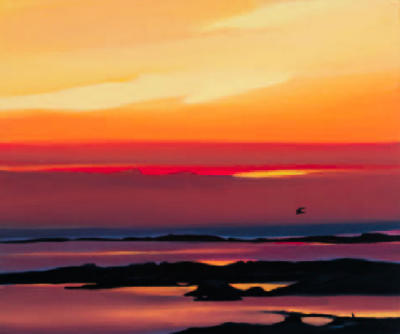
\includegraphics[width=\marginparwidth]{hist1.jpg}
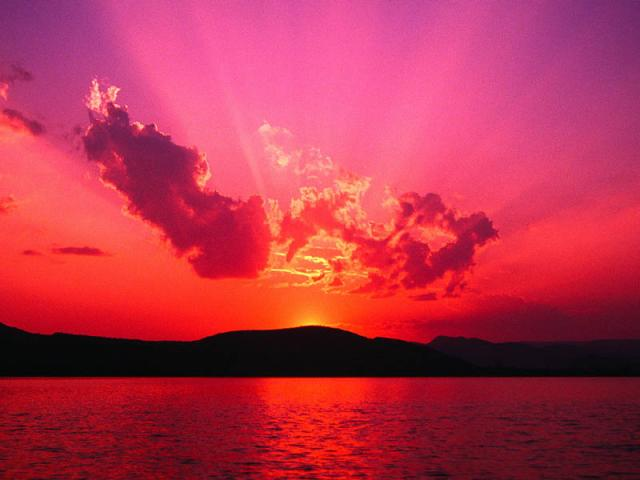
\includegraphics[width=\marginparwidth]{hist2.jpg}
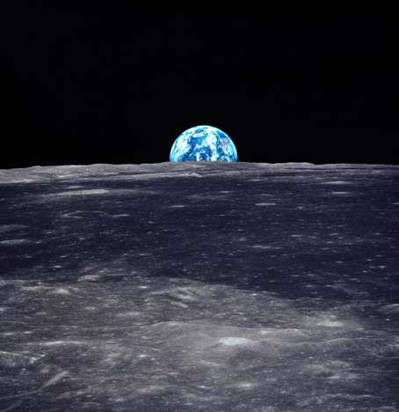
\includegraphics[width=\marginparwidth]{hist3.jpg}
}
\begin{lstlisting}[language=java]
URL[] imageURLs = new URL[] {
   new URL( "http://users.ecs.soton.ac.uk/dpd/projects/openimaj/tutorial/hist1.jpg" ),
   new URL( "http://users.ecs.soton.ac.uk/dpd/projects/openimaj/tutorial/hist2.jpg" ), 
   new  URL( "http://users.ecs.soton.ac.uk/dpd/projects/openimaj/tutorial/hist3.jpg" ) 
};
List<Histogram> histograms = new ArrayList<Histogram>();
for( URL u : imageURLs ) {
    HistogramModel model = new HistogramModel(4, 4, 4);
    model.estimateModel(ImageUtilities.readMBF(u));
    histograms.add( model.histogram );
}
\end{lstlisting}
We now have a list of histograms from our images.  The \verb+Histogram+ class extends a 
class called the \verb+MultidimensionalDoubleFV+ which is a feature vector represented 
by multidimensional set of double precision numbers.  This class provides us with a 
\verb+compare()+ method which allows comparison between two multidimensional sets of 
doubles. This method takes the other feature vector to compare against and a comparison 
method which is implemented in the \verb+DoubleFVComparison+ class.

So, we can compare two histograms using the Euclidean distance measure like so:
\begin{lstlisting}[language=java]
double distanceScore = histogram1.compare( histogram2, DoubleFVComparison.EUCLIDEAN );
\end{lstlisting}
This will give us a score of how similar (or dissimilar) the histograms are. It's useful
to think of the output score as a \textbf{distance} apart in space. Two very similar histograms 
will be very close together so have a small distance score, whereas two dissimilar 
histograms will be far apart and so have a large distance score.

The Euclidean distance measure is symmetric (that is, if you compare \verb+histogram1+ to 
\verb+histogram2+ you will get the same score if you compare \verb+histogram2+ to 
\verb+histogram1+) so we can compare all the histograms with each other in a simple, 
efficient, nested loop:
\begin{lstlisting}[language=java]
for( int i = 0; i < histograms.size(); i++ ) {
    for( int j = i; j < histograms.size(); j++ ) {
        double distance = histograms.get(i).compare( histograms.get(j), DoubleFVComparison.EUCLIDEAN );
    }
}
\end{lstlisting}

\section*{Exercises}
\subsection*{Exercise 1: Finding and displaying similar images}
Which images are most similar?  Does that match with what you expect if you look at the 
images?  Can you make the application display the two most similar images that aren't the same?

\subsection*{Exercise 2: Exploring comparison measures}
\raggedright
What happens when you use a different comparison measure (such as 
\verb+DoubleFVComparison.INTERSECTION+)?
